\section{Kompression}\label{sec:compression}

\subsection{Motivation}

Unabhängig davon, ob man eine Ausstellung in einem Museum gestaltet oder eine Webseite erstellt, lässt sich fast jede für Besucher oder Benutzer konzipierte Darstellung durch den Einsatz von Bildern aufwerten. Dieses lässt sich durch den Einsatz von 3D-Modellen, mit welchen der Benutzer durch Drehen, Zoomen, etc. interagieren kann, noch deutlich steigern. Abgesehen davon, dass dies in einer Ausstellung nur durch den Einsatz von Rechnern, wie beispielsweise von Tablets, möglich ist, sind damit jedoch einige technische Herausforderungen verbunden.

Einerseits erwartet der Benutzer ein möglichst realistisches Erlebnis, was nur durch hochaufgelöste 3D-Modelle und den damit einhergehenden großen Datenmengen möglich ist. Dennoch soll das Modell möglichst ohne Latenz angezeigt werden und flüssige Interaktion erlauben. Soll die Darstellung darüber hinaus auf einem mobilen Endgerät des Benutzers, wie beispielsweise einem Smartphone, stattfinden, das einerseits nur eingeschränkte Rechenkapazität bietet und auf das andererseits die gesamten Daten für jeden Benutzer separat übertragen werden müssen, entsteht hier ein Gegensatz, für den ein geeigneter Kompromis zu finden ist.

Dieser Kompromis besteht darin, die 3D"=Modelle nicht in der höchsten verfügbaren Auflösung dem Benutzer darzustellen, sondern in einer dem Anwendungsfall und dem Endgerät angemessenen Größe. Beispielsweise ist für eine ansprechende Anzeige auf einem Smartphone"=Bildschirm eine geringere Auflösung notwendig als auf der Workstation eines Museumsmitarbeiters mit entsprechend großem Bildschirm, die auch dementsprechend leistungsfähig ist, und über welche dieser Mitarbeiter das angezeigte Objekt erforschen möchte. Aus diesem Grund ist es sinnvoll, in der Medien-Datenbank die gespeicherten 3D"=Modelle in verschiedenen Auflösungen bereit zu halten, weshalb diese in der Regel beim Hochladen in die Datenbank automatisch komprimiert werden.

In diesem Kapitel wird nach einer kurzen Erläuterung der theoretischen Grundlagen auf die an die ViSIT"=Medien"=Datenbank angebundene Kompressions"=Komponente und deren Bedienung, die über eine Web-Oberfläche erfolgt, eingegangen. Abschließend wird die Schnittstelle, über welche die Kompressions"=Komponente unabhängig von der dafür verfügbaren Web-Oberfläche oder der ViSIT"=Medien"=Datenbank angesprochen werden kann, spezifiziert.

\subsection{Grundlagen}

Bei 3D-Modellen gilt es grundsätzlich zwischen der Geometrie, durch welche die Form der Oberfläche eines Objekts beschrieben wird, und der Textur, durch welche die Färbung der Oberfläche ausgedrückt wird, zu unterscheiden. Während die Geometrie obligatorisch für ein 3D-Modell ist, muss nicht zwangsläufig eine Textur existieren. Nicht jedes Digitalisierungsverfahren ist in der Lage, Texturdaten zu erfassen, wie beispielsweise ein Laserscanner. Im Folgenden werden Aufbau und Kompression dieser beiden Bestandteile eines 3D-Modells behandelt.

\subsubsection{Geometrie von 3D-Modellen}

Herkömmliche 3D"=Modelle, die ausschließlich die Oberfläche eines Objekts und nicht dessen Inneres beschreiben, bestehen aus Punkten im dreidimensionalen Raum, die \emph{Vertices} genannt werden. Diese Punkte werden zu Flächen, den sogenannten \emph{Faces} verbunden, wobei es sich hier in vielen Fällen um Dreiecke handelt. Die Anzahl der Ecken eines Faces wird als dessen \emph{Ordnung} bezeichnet. Die Kanten dieser Flächen, die Verbindungen zwischen zwei Vertices darstellen, werden \emph{Edges} genannt. Die Gesamtheit aller Vertices und Faces eines 3D"=Modells wird auch als \emph{Mesh} bezeichnet. Die soeben genannten Begriffe werden in Abbildung \ref{schlenke:fig:fundamentals:geo} grafisch dargestellt.

\begin{figure}
\centering
\subfloat[Vertex]{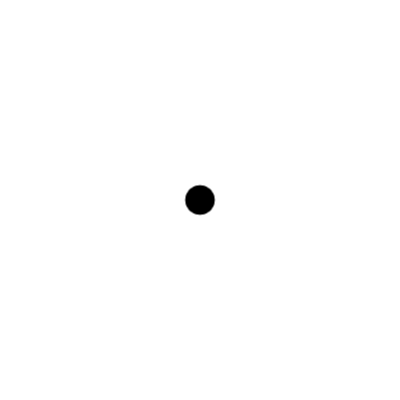
\includegraphics[width=0.25\textwidth]{Figures/schlenker/fundamentals/basicVertex.png}}
\qquad
\subfloat[Edge]{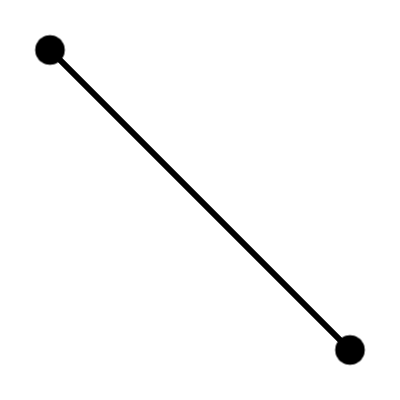
\includegraphics[width=0.25\textwidth]{Figures/schlenker/fundamentals/basicEdge.png}}
\qquad
\subfloat[Face]{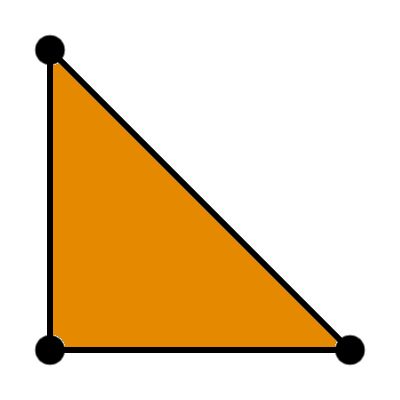
\includegraphics[width=0.25\textwidth]{Figures/schlenker/fundamentals/basicFace.png}}\\
\subfloat[Mesh]{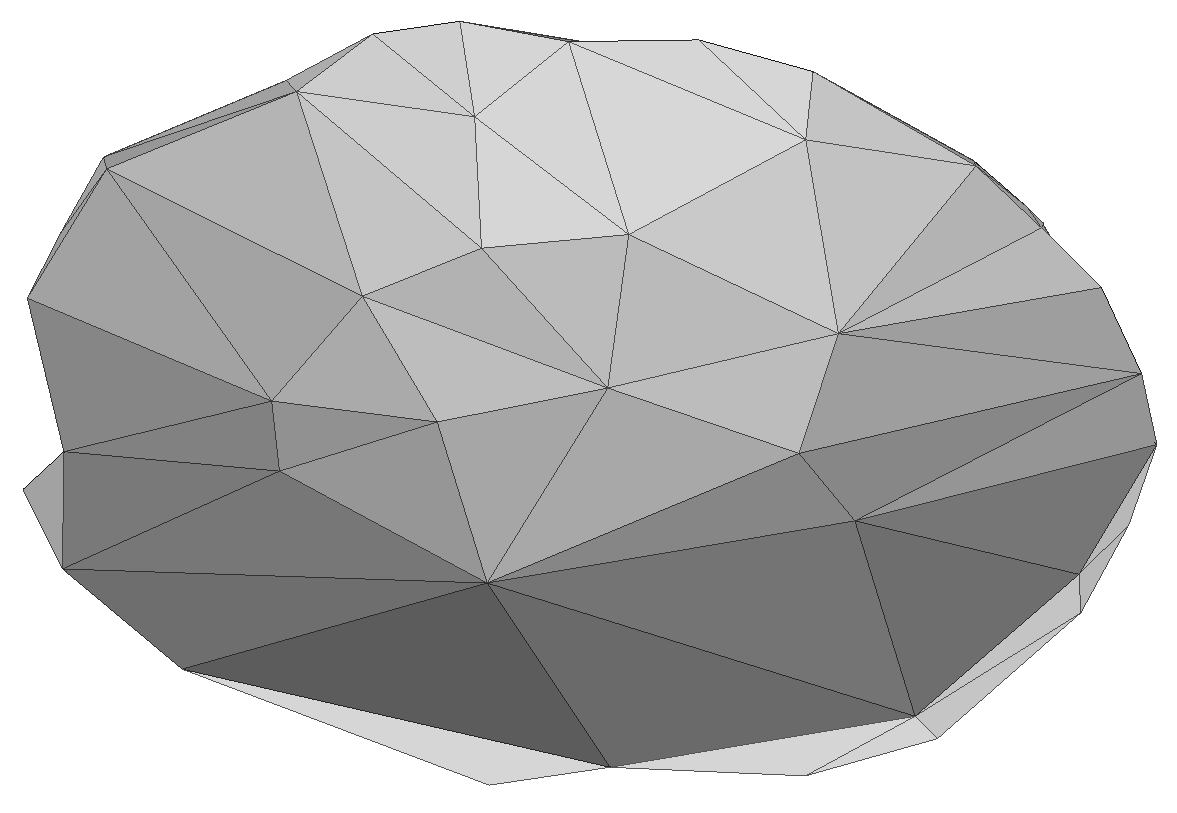
\includegraphics[width=0.70\textwidth]{Figures/schlenker/fundamentals/basicMesh.png}}
\caption{Grundlegende Elemente der Geometrie eines 3D-Modells}
\label{schlenke:fig:fundamentals:geo}
\end{figure}

Während bei einfachen Dateiformaten, wie beispielsweise dem STL-Format\footnote{\url{http://www.fabbers.com/tech/STL_Format}}, für jedes Face die Koordinaten eines jeden Eckpunkts separat gespeichert werden, wird die dadurch verursachte Redundanz zum Beispiel bei OBJ-Dateien\footnote{\url{http://www.martinreddy.net/gfx/3d/OBJ.spec}} vermieden, indem zunächst alle Vertices in Form der Koordinaten einmalig angegeben werden und anschließend bei der Definition der Faces auf diese Vertexdefinition indexbasiert zugegriffen wird.

[TODO manifold] \cite[S.~3]{botsch2010}

\subsubsection{Textur von 3D-Modellen}

Die Textur eines 3D"=Modells beschreibt dessen Färbung der Oberfläche, wodurch ihr eine äußerst wichtige Bedeutung für das visuelle Erlebnis beim Betrachten des Modells zukommt. Sie wird in der Regel getrennt von den eigentlichen Geometriedaten in einer separaten Bild"=Datei gespeichert. Für jedes Face wird dann durch die sogenannten \emph{Texturkoordinaten} festgelegt, welcher Ausschnitt des Textur-Bildes auf diesem Dreieck angezeigt wird. Pro Face werden also für jeden Eckpunkt zwei Werte gespeichert, durch welche eine eindeutige Position im Bild definiert wird. Da in der Regel bei den meisten Vertices alle angrenzenden Faces die gleichen Texturkoordinaten verwenden, wird dieses Paar von Werten beispielsweise bei OBJ-Dateien nur einmal gespeichert, worauf anschließend bei der Beschreibung der Faces indexbasiert zugegriffen wird.

Manchem Leser stellt sich hier die Frage, ob generell die Verwendung von einem Paar Texturkoordinaten pro Vertex, welches dann für alle angrenzenden Faces verwendet wird, nicht ausreichend wäre. Hier spielt jedoch die Geometrie des 3D"=Modells, genauer deren \emph{Topologie}, eine wichtige Rolle. Entspricht diese einer (verzerrten) Ebene, so wäre diese Vereinfachung in der Tat ausreichend. Betrachtet man aber beispielsweise eine Kugel, so lässt sich das zweidimensionale Bild nicht über die Kugel legen, ohne dass eine Kante entsteht, an welcher mindestens zwei Ränder des Bildes aneinandergrenzen. Genau entlang dieser Linie, dem sogenannten \emph{Texture Seam}, befinden sich dann die Vertices, für welche je nach angrenzendem Face verschiedene Texturkoordinaten verwendet werden müssen. Unabhängig von der soeben dargelegten Notwendigkeit dieser Texture Seams lässt sich durch eine sinnvolle Unterteilung der Textur auch die Qualität erhöhen, indem für alle Bereiche des 3D"=Modells eine ähnliche Auflösung verwendet wird und durch starke Streckungen oder Stauchungen verursachte Verzerrungen der Textur auf dem Modell minimiert werden.

\subsubsection{Kompression der Geometrie}

Eine der wichtigsten Herangehensweisen zur Kompression von 3D"=Modellen ist die Reduktion von Vertices und damit einhergehend die Verringerung der Anzahl an Faces. Ausgehend von einem hoch aufgelösten Modell mit einer hohen Anzahl an Vertices ist die auf den ersten Blick einfachste Vorgehensweise das Entfernen eines möglichst unwichtigen Vertices. Das dadurch entstehende Loch im Mesh muss anschließend geschlossen werden. Dadurch entsteht jedoch im Allgemeinen ein Face mit einer höheren Ordnung, was oft unerwünscht ist. In diesem Fall muss das entstehende Loch mit Dreiecken gefüllt werden, wofür es keine eindeutige und daher auch unterschiedlich gute Lösungen gibt. Stattdessen verwenden viele Kompressionsverfahren, wie auch der in dieser Kompressions-Komponente verwendete Algorithmus, sogenannte \emph{Edge-Collapse}-/\emph{Half-Edge-Collapse}-Operationen.

Bei einer solchen Edge-Collapse-Operation, wie sie in Abbildung [TODO] dargestellt ist, werden zwei durch ein Edge verbundene Vertices zu einem neuen Vertex verschmolzen. Dabei degenerieren die an dieses Edge angrenzende Faces und werden entfernt. Zusätzlich lassen sich neben dem kontrahierten Edge noch weitere Edges entfernen. Entspricht der Mesh lokal einer Mannigfaltigkeit, werden durch eine Edge-Collapse-Operation also zwei Faces, drei Edges und ein Vertex entfernt. Vor dem Durchführen einer derartigen Operation muss jedoch überprüft werden, ob die in \cite[S.~118f]{botsch2010} erläuterte \emph{Link Condition} erfüllt ist, da andernfalls die Topologie des Meshes durch die Operation verändert werden kann. Entspricht der neue Vertex einem der beiden ursprünglichen Vertices, so spricht man von einem Half-Edge-Collapse.

Es verbleibt jedoch die Frage, welche Paare von Vertices verschmolzen werden sollen. Hierfür wird in \cite{garland1997} ein Verfahren vorstellt, das mithilfe von Quadriken jeder möglichen Edge-Collapse-Operation einen Wert für die damit verbundenen Kosten zuweist. Iterativ werden nun die Vertices aus Operationen mit den geringsten Kosten verschmolzen, woraufhin die Kosten der Operationen, die sich auf die umliegenden Vertices beziehen, aktualisiert werden müssen.

Der Algorithmus aus \cite{garland1997} ist jedoch nur auf nicht-texturierte Meshes anwendbar. Möchte man dieses Verfahren verwenden, um 3D"=Modelle mit Textur zu komprimieren, so müssen einerseits die Verschmelzungsoperationen auch auf die Texturkoordinaten angewandt werden, was insbesondere entlang von Texture Seams eine sehr sorgfältige Implementierung erfordert, andererseits müssen aber auch dieses Texturkoordinaten in die Berechnung der Kosten für die jeweilige Operation miteinbezogen werden. Abweichungen in der resultierenden Oberfläche des 3D"=Modells haben hier Verzerrungen in der Textur zur Folge. Dies gilt auch für Texture Seams, bei welchen es darüber hinaus nicht vermeiden lässt, dass auch Bereiche der als Textur verwendeten Bilddatei für die Einfärbung der Faces verwendet werden, die im ursprünglichen Modell überhaupt nicht parametrisiert waren und somit beliebigen Inhalt aufweisen können. Es empfiehlt sich daher, die Ränder der Bereiche in der Bilddatei mit einem ähnlichen Farbton wie die eigentliche Textur zu färben, was bei den meisten Textur erzeugenden Programmen automatisch geschieht. Die daher notwendige Erweiterung des bestehenden Kompressions-Algorithmus auf texturierte Meshes wird in \cite{garland1998} vorgenommen, wobei Texture Seams dort kaum behandelt werden. Die für die Kompressions-Komponente erstellte Implementierung behandelt jedoch auch diese Bereiche auf eine sinnvolle Art und Weise.

\subsubsection{Kompression der Textur}

Während die Kompression der Modellgeometrie insbesondere bei texturierten Meshes nichttrivial ist, gestaltet sich die Kompression der Texturdaten relativ einfach. Die Textur wird in einer herkömmlichen Bilddatei gespeichert, deren Dateigröße direkt von der Auflösung des darin gespeicherten Bildes abhängt. Wird die Auflösung des Bildes verringert, was der Funktionsumfang eines jeden brauchbaren Bildbearbeitungsprogramms zulässt, schlägt sich dies auch in der Größe der Texturdatei nieder. Darüber hinaus sind weitere aus der Bildverarbeitung bekannte Kompressionsverfahren einsetzbar, wie zum Beispiel die JPEG-Komprimierung [TODO Referenz]

Allerdings muss darauf geachtet werden, dass die zusammen mit der Modellgeometrie gespeicherten Texturkoordinaten auch nach der Kompression der Textur wohldefiniert sind. Besonders angenehm ist hier jedoch die Tatsache, dass diese Texturkoordinaten sich nicht auf die Pixel beziehen, sondern stets im Interval von 0 bis 1 liegen, wobei sich 0 auf den oberen bzw. linken Rand und  1 auf den unteren bzgl. rechten Rand der Texturdatei bezieht. Aus diesem Grund sind die Texturkoordinaten gänzlich unabhängig von der Auflösung der die Textur beinhaltenden Bilddatei und diese Datei kann ohne Modifizierung der Geometriedatei komprimiert werden. Diese Aussage gilt nicht nur für die Anpassung der Auflösung, sondern auch für andere Kompressionsverfahren aus der Bildverarbeitung.